\lecture{9}{2025-03-18}{Introduction to cryptography}{}

\chapter{Cryptography}
    \section{One-Time pad, Perfect Secrecy, Public-Key}
    

\begin{parag}{Why cryptography}
    cryptography gives us the tools to:
    \begin{itemize}
        \item authenticate the sender and the receiver
        \item verify the integrity of the message
        \item keep the message confidential
    \end{itemize}
\end{parag}
\begin{parag}{Basic setup for condidentiality}
    \begin{center}
        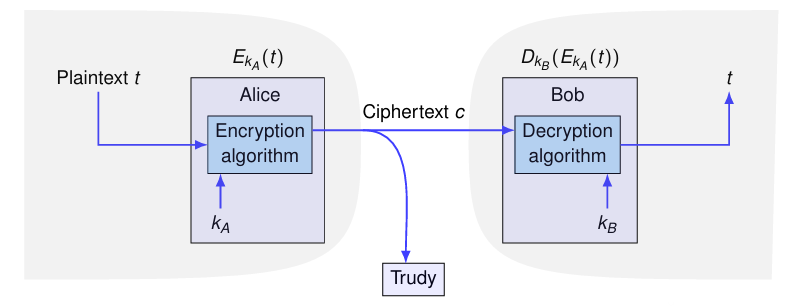
\includegraphics[scale=0.6]{12025-03-18.png}
    \end{center}
   Here Alice want to sent the plaintext $t$ to Bob:
   \begin{itemize}
       \item She encrypts $t$ using her key $k_A$. Theresult is the ciphertext $c = E_{k_A}(t)$
       \item She sends $c$ to Bob over a public channel
       \item Bob decrypts $c$ using his key $k_B$. The result is $D_{k_B}(E_{k_A}(t)) ) t$
       \item For Trudy, it is nearly impossible to recover $t$ from $c$ without knowing $k_B$
   \end{itemize}
\end{parag}
\begin{parag}{Basic Terminology}
    \begin{itemize}
        \item pleintext, ciphertext (also called cryptogram), key, encrypter, decrypter
        \item cryptography: the art of composing cryptograms
        \item cryptanalysis the art of breaking cryptograms
        \item a cryptanalyst has broken the system when he cann quickly determine the plaintext from the cryptogram, no matter what key is used
        \item attacker: same as cryptanalyst
    \end{itemize}

\end{parag}
\begin{parag}{Ancient cryptography}
    \begin{subparag}{Caesar's cipher}
        Suppose that we are using the English alphabet augmented by a few special characters, "space", "comma", and "period".\\ An alphabet of $29$ characters, represented by the integers $0, 1 , \dots, 28$
        \begin{itemize}
            \item The key $k$ is an integer between $0$ and $28$, known to Alice and Bob and to nobody else.
        \item The encryption algorithm substitues the $i$-th letter of the alphabet with the $(i + k)th$ letter $(\mod 29$)
        \item The decryption algorithm substitues the $j$-th letter with the $(j-k)$-th $\mod 29$ 
    \end{itemize}
       Therefore, here the secrecy of the message rely only on the secrecy of the algorithm. 
    \end{subparag}
    \begin{subparag}{Various attacks possible}
        We distinguish between the following attacks:
        \begin{itemize}
            \item \important{ciphertext-only}: one or more cryptograms available to the cryptanalyst know to have been encrypted with the same key
            \item \important{known plaintext}: the cryptanalyst has one or more plaintext and the resulting cryptograms, know to have been encrypted with the same key
            \item \important{chosen plaintext} for any plaintext that he requires, the cryptanalyst can obtain the cryptogram under the same key
        \end{itemize}
        Ideally, a cryptographic system should be secure against a chosen plaintext attack, At the very least, it should be secure against a cipthertext-only attack.
    \end{subparag}
    However with a computer, the key can easily be found using the letter-frequency attack. The question now is how to make the letter frequency attack unfruitful?
\begin{subparag}{Example (Vigenère's cipher with an $n$-length key}
    \begin{itemize}
        \item Chosen plaintext attack: encode the same letter until you have the $n-$length key
        \item \important{known plaintext attack} compare input/output until you have the $n$-length key
        \item \important{ciphertext-only attack}
            \begin{itemize}
                \item brute force approach: try all $29^n$ keys is you know $n$
                    \begin{itemize}
                        \item for $n = 21$ the number of key is $5.13^{30}$
                        \item for $n = 100$, the number of keys is $1.73^{146}$
                    \end{itemize}
                \item If you know $n$, you can partition input/output into $n$ parts, each of which is a Caesar cipher with its own key
                \item Letter frequency approach: effective if the plaintext-length to key-length ration is sufficiently large
            \end{itemize}
    \end{itemize}
\end{subparag}
\end{parag}

\begin{parag}{The one-time pad}
    Preliminary assumptions
    \begin{itemize}
        \item The plaintext $t$, the key $k$ and the cryptogram $c$ are n-length binary sequences over the alphabet $ \mathcal{A} = \{0, 1\}$
        \item The key $k$, is produced by selecting each bit independently and with uniform distribution
        \item Alice and Bob use a private chanel to exchange the key ahead of time
    \end{itemize}
    \textbf{Encryption}
    \begin{align*}
        c = t \oplus k
    \end{align*}
    \textbf{Decryption}
    \begin{align*}
        c \oplus k = (t \oplus k) \oplus k = t \oplus ( k \oplus k) = t
    \end{align*}
    
    

\end{parag}



\begin{parag}{Perfect secrecy}
    \begin{definition}
        A cryptosystem has \important{perfect secrecy} if the plaintext $T$ and the cryptogram $C$ are statistically independent
    \end{definition}
    Perfect secrecy is the ultimate kind of security against a ciphertext-only attack: The attacker cannot do better than guessing the plaintext $T$

\end{parag}
\begin{parag}{Perfect secrecy of the one time pad}
    \begin{itemize}
        \item The $n$-length key $k$ is selected at random (uniform distribution ober $\{0,1\}^n$)
        \item The key $k$ and the message $t$ are selected independently
        \item The ciphertext is $c = t \oplus k$
           \begin{align*}
               p_{C \mid  T}( c \mid  t) = p_{K \mid  T}( c \ominus t \mid  t) = p_K ( c \ominus t ) = \frac{1}{2^n}
           \end{align*}
    \end{itemize}
    Hence $C$ and $T$ are independent: knowledge of $C$ is useless in guessing $T$
\end{parag}
\begin{parag}{Weakness of the one time pad}
    \begin{subparag}{Example}
        A cryptanalyst that has the plaintext $t$ and the corresponding cryptogram $c$ immediately gets the key:
        \begin{align*}
            k = c \ominus t
        \end{align*}
        Hence the pad (the key) should be used only once
    \end{subparag}
    \begin{subparag}{Pros and Cons of one time pad}
        \textbf{Pros}
        \begin{itemize}
            \item Very simple algorithm
            \item as secure as it gets against a ciphertext-only attack and key used one
            \item of instructional value to prove that the perfect secrecy is possible
        \end{itemize}
        \textbf{Cons}
        \begin{itemize}
            \item The key is as long as the plaintext (this is fundamental, see later)
            \item The key needs to be exchanged ahead of time over a private chanel
            \item a ciphertext-only attack can break the system if the key is used twice (see homework)
            \item a known plaintext attack reveals the key
        \end{itemize}
        The "one-time pad" has been used extensively in diplomatic and espionage circles
        
    \end{subparag}

\end{parag}
\begin{parag}{Perfect secrecy requires high entropy keys}
    The following theorem makes no assumption on the encryption algorithm:
    \begin{center}
        \begin{tikzpicture}
            \draw[](0, 0) rectangle(2, 3) node at (0.5, 1.5){encryption};
        \draw[<-](2, 2) -- (2.5, 2) node at (2.75, 2) {$t$};
        \draw[->](2, 0.5) -- (2.5, 0.5) node at (2.75, 0.5){$c$};
        \draw[->](-0.5, 1.5) -- (-0, 1.5) node at(-0.75, 1.5){$k$};
        \end{tikzpicture}
        
        
    \end{center}
    
    \begin{theoreme}
        Perfect secrecy implies:
        \begin{align*}
            H(T) \leq H(K)
        \end{align*}
        
    \end{theoreme}
   \begin{subparag}{Proof}
       Perfect secrecy $H(T) = H(T \mid  C)$ and decodability $(H(T \mid  K, C) = 0)$ imply:
       \begin{align*}
           H(T) &= H(T \mid  C)\\
                &\leq H(T, K \mid C)\\
                &= H(K \mid  C) + H(T \mid  K, C)\\
                 &= H(K \mid  C)\\
                &\leq H(K)
       \end{align*}
       Given  $T, K, C$ we search for the entropy:
       \begin{align*}
           H(t, k, c) &= H(c) + \overbrace{H(t \mid  c)}^{=H(t)} + H(k \mid  t, c) \\
                      &= H(c) + H(k \mid  c) + \underbrace{H(t \mid  k, c)}_{= 0} \\
                      &\implies H(t) + H(k, \mid  t, c) \leq h(k \mid  c)
       \end{align*}
This implies:
\begin{align*}
    H(t) + \underbrace{H(k \mid t, c)}_{ \geq 0} \leq H(k)
\end{align*}
Because if we take out the \textit{"Knowing c"} we cannot have some bigger. 
Therefore:
\begin{align*}
    H(t) \leq H(k)
\end{align*}



   \end{subparag}
   \begin{framedremark}
       Entropy plays a key role also in cryptography
   \end{framedremark}
   
\end{parag}

